\chapter{Experimento}\label{chapter:experimento}

Neste capítulo é apresentado o experimento que realizado para a avaliação da proposta apresentada no Capítulo \ref{chapter:proposta}.
Para avaliar a proposta deste trabalho foi utilizada uma avaliação pela perspectiva do usuário, que segundo a definição de
\citeonline{shani2011evaluating} se encaixa em um Estudo com usuários. O algoritmo proposto será incorporado ao ambiente
\adaptweb e avaliado em uma situação real de uso em um Minicurso de Algoritmos desenvolvido por \citeonline{santos2017addie}.
Na Seção \ref{section:planejamento-experimento} é descrito o ambiente \adaptweb no qual a proposta será incorporada,
as mudanças realizadas no ambiente para o experimento, o objetivo do experimento e o teste piloto realizado. A Seção
\ref{section:execucao-experimento} descreve o experimento que foi realizado e Seção \ref{section:analise-experimento} apresenta
as análises estatísticas realizadas no questionário de satisfação e no uso do Sistema de Recomendação (SR).

\section{Planejamento}\label{section:planejamento-experimento}

\subsection{Descrição do Ambiente \adaptweb}

O \adaptweb (Ambiente de Ensino-Aprendizagem Adaptativo na Web) é um sistema open source
que consiste em um AVA capaz de adaptar o conteúdo, a apresentação e a navegação em determinado curso às características
e preferências do aluno \cite{gasparini2009adaptweb}. A Subseção \ref{subsection:estrutura-adaptweb} apresenta a Estrutura Geral do
\adaptweb.

\subsubsection{Estrutura do \adaptweb}\label{subsection:estrutura-adaptweb}

A estrutura do \adaptweb é composta por quatro módulos: (1) o módulo de autoria; (2) o
módulo de armazenamento em XML (Extensible Markup Language); (3) o módulo de adaptação do conteúdo baseado no modelo do
usuário e (4) o módulo de interface adaptativa \cite{gasparini2003interface}, conforme pode ser visto na Figura
\ref{fig:adaptweb-arquitetura}.

\begin{figure}[htb]
  \caption{\label{fig:adaptweb-arquitetura}Estrutura do \adaptweb}
  \begin{center}
      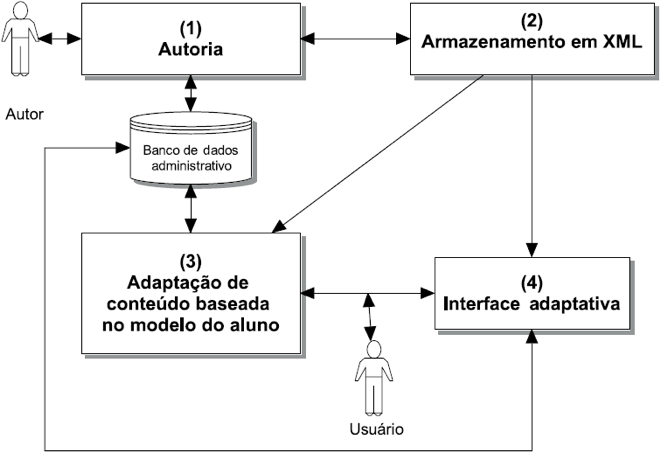
\includegraphics[scale=1.0]{./Figuras/adaptweb-arquitetura.png}
  \end{center}
  \legend{Fonte: \citeonline{gasparini2003interface}}
\end{figure}

O módulo de autoria (1) consiste na organização do conteúdo instrucional a ser disponibilizado para o aluno, sendo que
este conteúdo pode ter arquivos classificados como conceito, exemplos, exercícios e materiais complementares
\cite{gasparini2003interface}. Ao criar um conteúdo no sistema, o autor pode definir para quais cursos e disciplinas
deseja que o conteúdo ou arquivo esteja disponível. Isto significa que um aluno de um Curso X e de outro Curso Y,
matriculados em uma mesma disciplina, podem ter conteúdos distintos, conforme definido pelo professor. Por exemplo, a
disciplina de Cálculo I pode ser oferecida para os cursos de Ciência da Computação e Engenharia Elétrica e sua
abrangência e profundidade pode ser distinta para cada curso.

Em \citeonline{de2015sistema}, foi proposto uma nova categoria para os conteúdos chamada Links de Apoio. Esses Links de Apoio
são links externos ao ambiente \adaptweb que são cadastrados pelo professor como um
material alternativo de estudo e não estão diretamente atrelados á nenhum conceito em específico. O objetivo foi criar
uma nova categoria de materiais que poderia ser recomendada para o usuário a qualquer momento de sua interação.

O módulo de armazenamento em XML (2) é responsável por organizar os conteúdos e arquivos disponibilizados pelo autor em
um arquivo XML \cite{gasparini2003interface}. É utilizada a representação através de XML devido à sua alta
flexibilidade, oferecendo a estruturação dos documentos de forma independente da apresentação.

O módulo de adaptação do conteúdo baseado no modelo do aluno (3) é responsável por adaptar o conteúdo da disciplina
para cada curso. Por fim, o módulo de interface adaptativa (4) é responsável pela adaptação da navegação e da
apresentação da interface do ambiente de acordo com o curso, preferências do modo de navegação (modo tutorial ou livre)
e o conhecimento do usuário \cite{gasparini2003interface}.

\subsubsection{Sistema de Recomendação no \adaptweb}

Na Subseção \ref{subsection:estrutura-adaptweb} foi apresentada a estrutura do ambiente \adaptweb, que possui quatro categorias
de materiais para cada conteúdo. Além disso, existe uma outra categoria chamada Links de Apoio com o propósito de ser um
material auxiliar e que pode ser recomendado a qualquer momento para o usuário.

Fazendo uma relação da estrutura do \adaptweb com o algoritmo proposto no Capítulo \ref{chapter:proposta}, os itens de
das categorias Conceito, Materiais Complementares e os próprios Links de Apoio serão considerados para a composição do perfil do usuário. Todos os
materiais acessados em cada uma das categorias é representado através das palavras-chave, e
essas palavras-chave farão parte do perfil do aluno a partir do momento em que este acessar o material. Já para os itens
recomendados, apenas os Links de Apoio serão utilizados.

Como no ambiente \adaptweb as palavras-chave para o itens podem ser cadastradas pelo professor da disciplina, não será
utilizada nenhuma técnica para captura automática das palavras-chave. Para a representação dos materiais envolvidos no
processo de recomedanção (i.e., Conceitos, Materiais Complementares e Links de Apoio) foi criado um Dicionário de Palavras-Chave
com as possíveis palavras a ser utilizadas. Esse Dicionário foi essencial para o funcionamento do SR, pois garante que as
palavras-chave presentes nos materiais que são similares também serão similares. Isso evita a necessidade de lidar com palavras-chave
sinônimas ou a variação de singular e plural, já que as palavras-chave que podem ser utilizadas para representar os materiais
são restritas às presentes no dicionário.

O Dicionário completo pode ser visto no Apêndice \ref{ape:dicionario-palavras-chave}. A criação do Dicionário foi validado
por um aluno do Mestrado em Ensino de Ciências, Matemática e Tecnologias que também é professor da disciplina de
Algoritmos no SENAC-SC. O professor teve acesso ao Minicurso de Algoritmos utilizado no experimento
e teve o papel de avaliar o Dicionário criado e acrescentar mais palavras para agregar conjunto de palavras-chave.

Depois de criado e validado o Dicionário, foi realizada a associação de forma manual entre cada material dos Conceitos,
Materiais Complementares e Links de Apoio com as palavras-chave do Dicionário. No total, 51 Conceitos, 28 Materiais
Complementares e 108 Links de Apoio foram analisados. O resultado dessa associação pode ser visto no Apêndice \ref{ape:palavras-chave-materiais}.

O Sistema de Recomendação (SR) irá buscar, com base nos itens acessados pelo aluno, os Links de Apoio mais adequados
para a recomendação e irá apresentar através de uma lista de itens. A forma de apresentação das Recomendações é discutida
em mais detalhe na Subseção \ref{subsection:apresentacao-recomendacoes}.

\subsubsection{Apresentação das Recomendações}\label{subsection:apresentacao-recomendacoes}

A lista de recomendações neste trabalho será apresentada ao aluno na tela principal do ambiente do aluno. Dessa forma,
quando o SR possuir itens para recomendar para o usuário esses itens aparecem em uma lista logo abaixo do conteúdo que
ele estiver visualizando no momento, independente se o aluno estiver na tela de Conceito, Exercícios, Exemplos ou
Materiais Complementares. Na Figura \ref{fig:adaptweb-proposta-recomendacao} pode-se observar a tela inicial do ambiente do
aluno, onde estão destacadas as seguintes áreas: (1) Menu de navegação pelos tópicos; (2) Categorias dos materiais dentro
do ambiente; (3) Interface das recomendações; (4) Mapa da disciplina; (5) Ajuda. As recomendações podem ser apresentadas ao usuário no momento em que este estiver acessando
quaisquer itens que sejam da categoria Conceito e Materiais Complementares, assim que o SR possuir itens relevantes para recomendar.

\begin{figure}[htb]
  \caption{\label{fig:adaptweb-proposta-recomendacao}Proposta de Interface de Recomendação}
  \begin{center}
      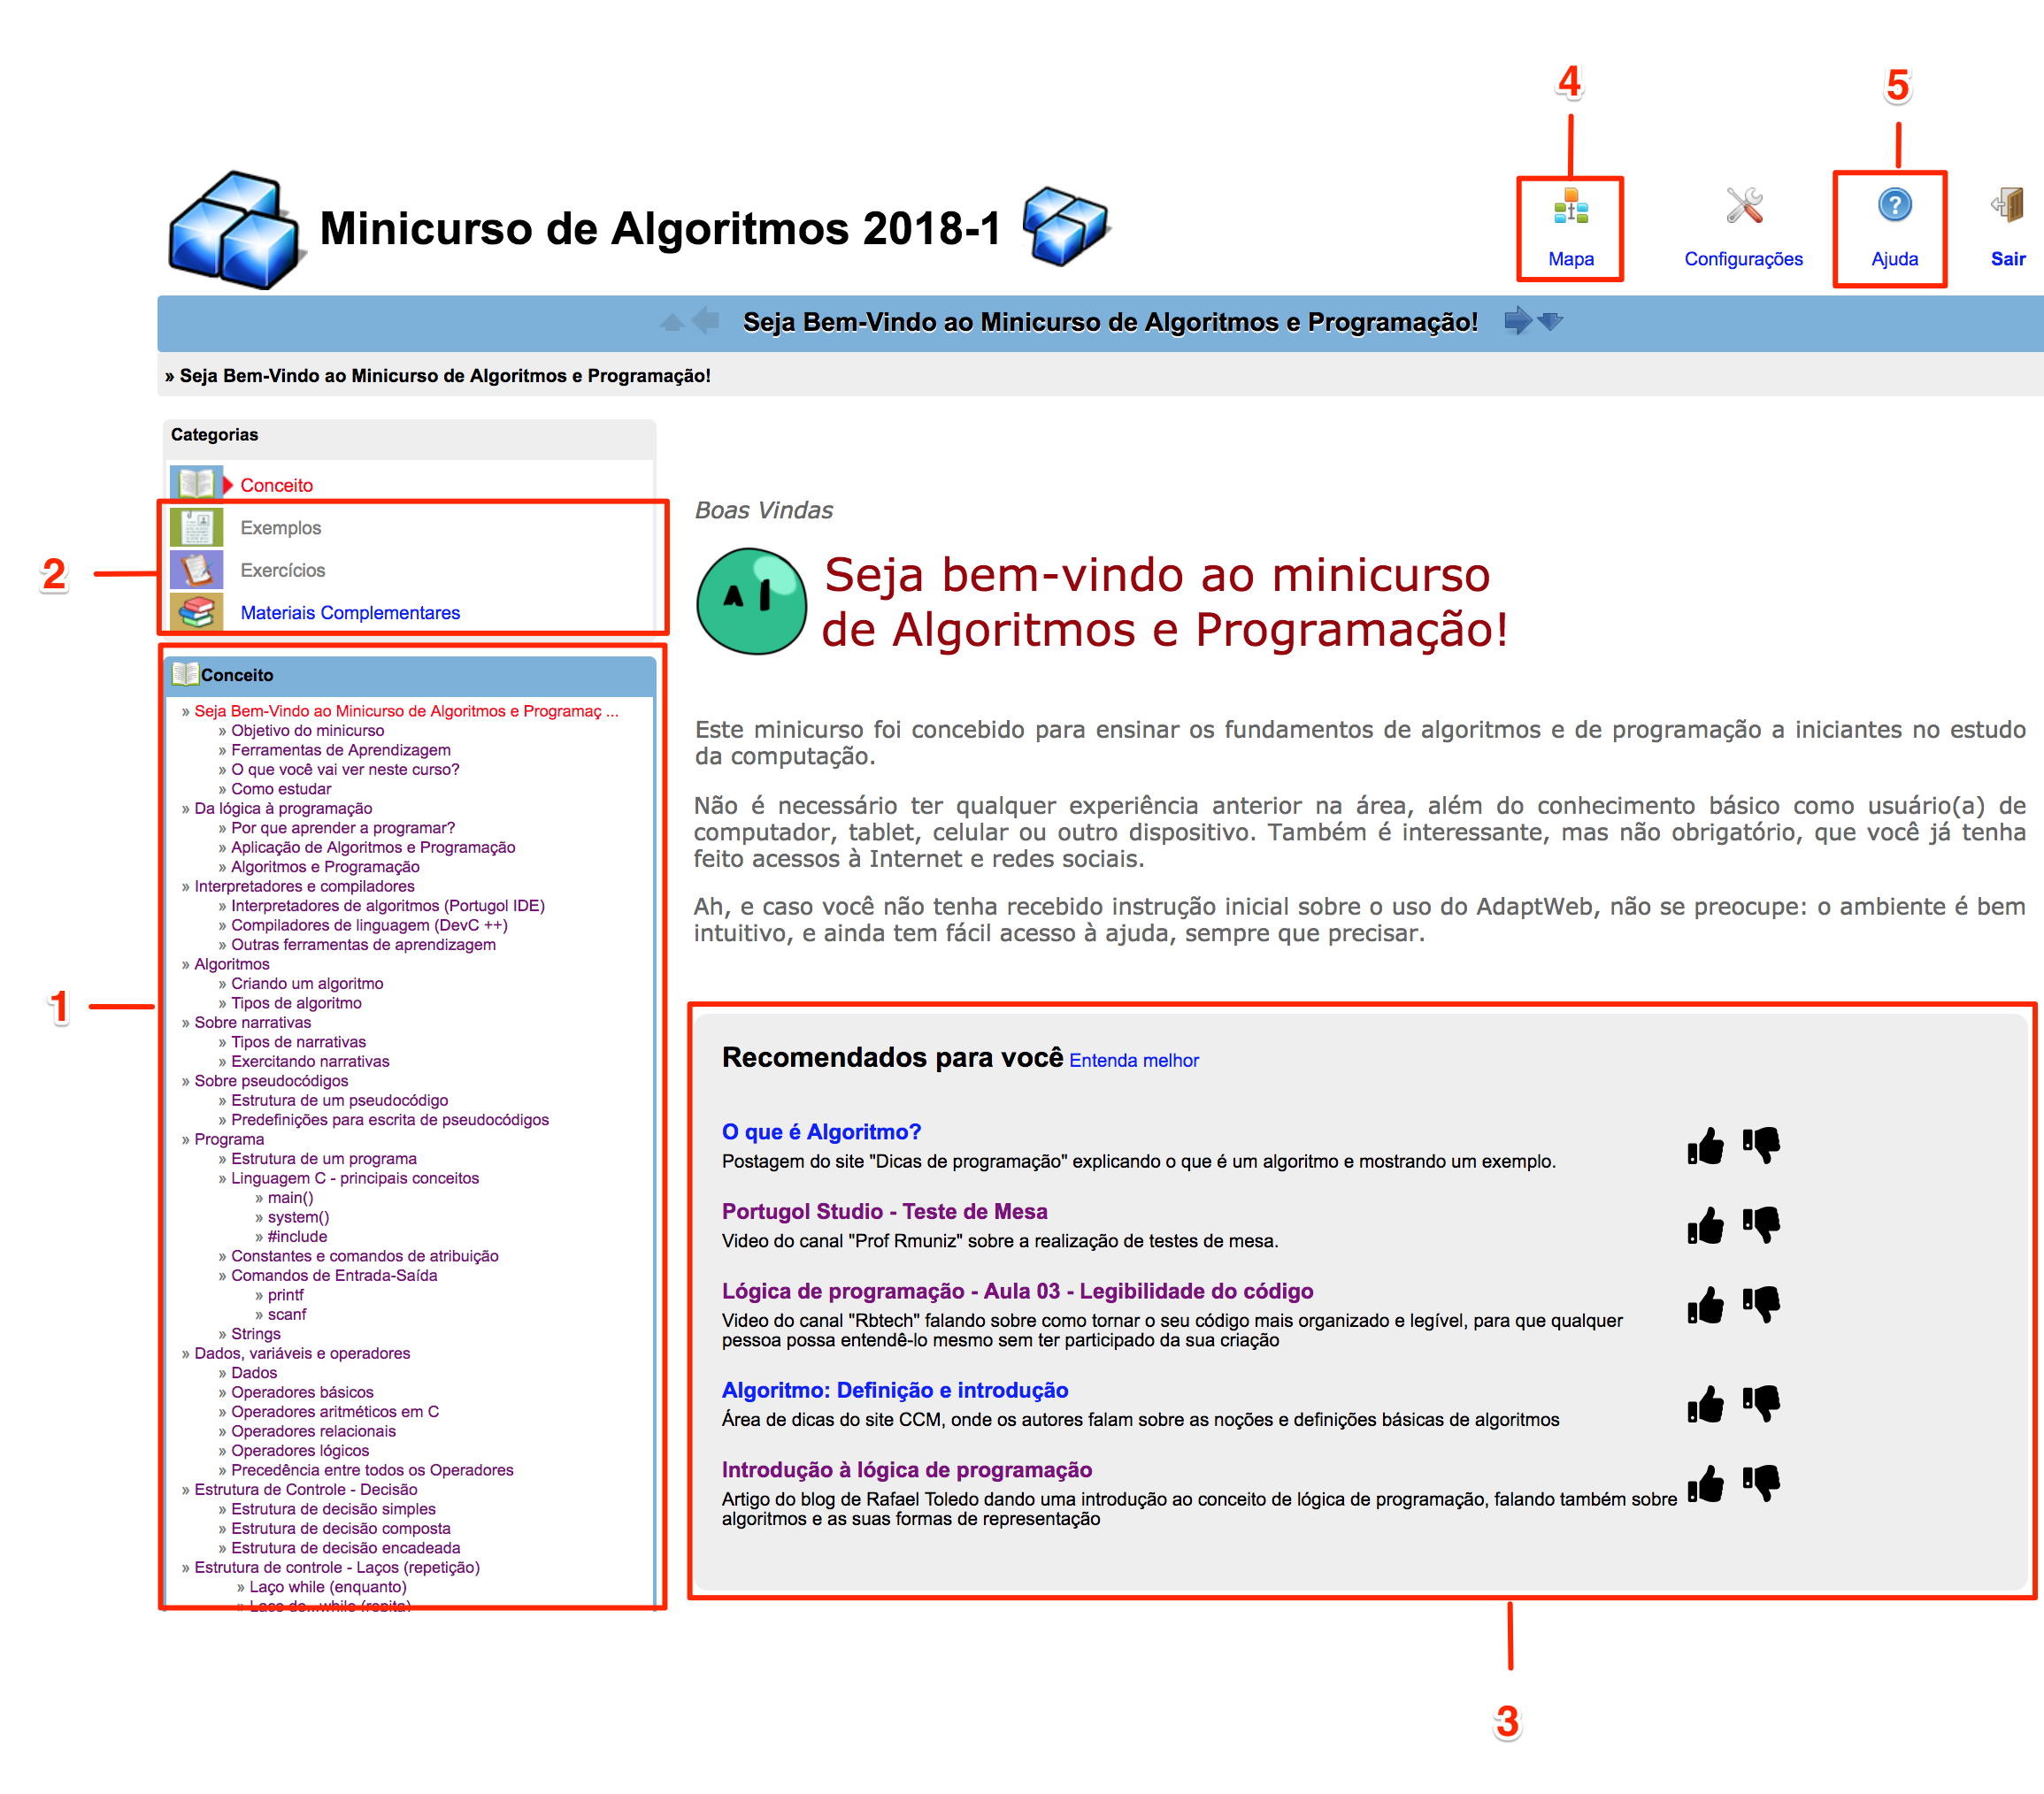
\includegraphics[scale=0.4]{./Figuras/interface-recomendacao.png}
  \end{center}
  \legend{Fonte: O autor.}
\end{figure}

Como visto na imagem, as principais informações dos Links de Apoio recomendados apresentados para o aluno são: Link, Nome do Link, Descrição e a possibilidade de avaliar o item
positivamente ou negativamente. A avaliação feita pelo usuário não é considerada pelo algoritmo de recomendação, sendo que os itens acessados pelo
usuário são considerados como do seu interesse. Como trabalho futuro é possível incorporar a avaliação na recomendação, e.g.,
não tornar a recomendar itens que foram avaliado com notas baixas ou apenas considerar para o algoritmo Baseado em Conteúdo
os itens avaliados positivamente. \citeonline{pu2012evaluating} afirmam que enquanto recomendar um item apenas é pouco, recomendar mais do que cinco itens
aumenta a dificuldade de escolhar do usuário. Por isso, a quantidade máxima de itens recomendadas para o usuário em cada
recomendação é de cinco itens.

Para cumprir o requisito de Explicação das recomendações citada por \citeonline{pu2012evaluating}, foi adicionado o
botão de "Entenda melhor" que tem por objetivo explicar ao usuário como a lista de itens foi gerada. Ao entender o
funcionamento do algoritmo de recomendação o usuário tem a possibilidade aprimorar o seu perfil para personalizar as
recomendações recebidas. Na Figura \ref{fig:adaptweb-proposta-explicacao} está um protótipo da explicação da recomendação
mostrada para o aluno.

\begin{figure}[htb]
  \caption{\label{fig:adaptweb-proposta-explicacao}Explicação da recomendação}
  \begin{center}
      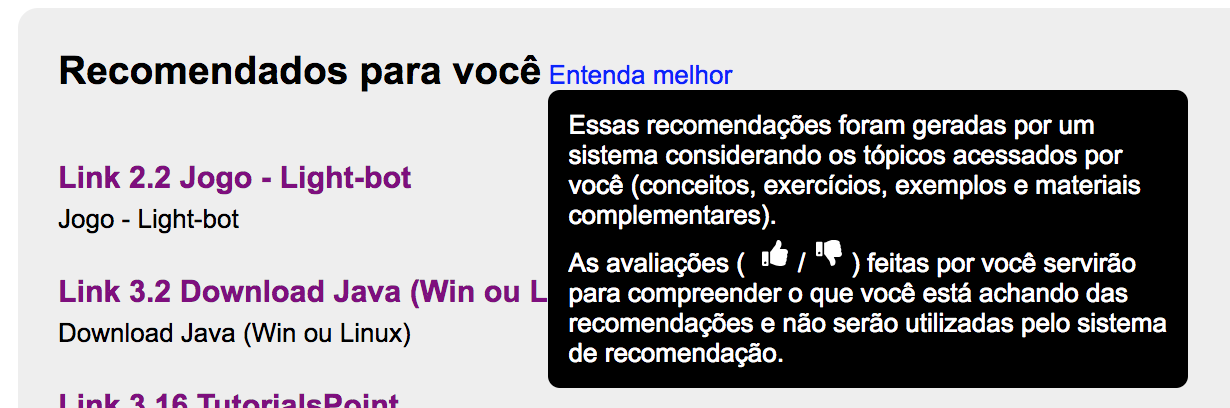
\includegraphics[scale=0.6]{./Figuras/explicacao-das-recomendacoes.png}
  \end{center}
  \legend{Fonte: O autor.}
\end{figure}

\subsection{Definição do experimento}\label{subsection:definicao-experimento}

O experimento proposto neste trabalho visa avaliar a experiência dos alunos ao interagir com o SR proposto, se comparado a um SR
utilizando a abordagem Baseada em Conteúdo tradicional. Este experimento foi
baseado nas seguintes hipóteses:

\begin{itemize}
\item \textbf{H\textsubscript{0}:} Não há diferenças na percepção do usuário da qualidade das recomendações recebidas utilizando a abordagem
Baseada em Conteúdo tradicional e a proposta desse trabalho.
\item \textbf{H\textsubscript{1}:} Há diferenças na percepção do usuário da qualidade das recomendações recebidas utilizando a abordagem
Baseada em Conteúdo tradicional e a proposta desse trabalho.
\end{itemize}

Para a execução do experimento, o SR proposto foi comparado a abordagem Baseada em Conteúdo tradicional utilizando uma
estratégia \textit{Between Subjects}, i.e., os alunos foram divididos em dois grupos e cada grupo utilizou apenas
um dos sistemas. Para garantir que a única variável seja o SR utilizado, ambos os grupos irão utilizar a mesma
interface proposta para as recomendações.

O experimento foi realizado através do Minicurso de Algoritmos e Linguagem de Programação, o qual teve seu design instrucional realizado por \citeonline{santos2017addie}.
Foram convidados a participar alunos de todos os cursos do Centro de Ciências Tecnológicas (CCT) da Universidade do
Estado de Santa Catarina (UDESC), sendo que todos os cursos do CCT possuem essa disciplina na grade curricular. Os convites
foram realizados em todas as salas das disciplinas de Algoritmos (ALG), Algoritmos e Linguagem de Programação (ALP), Linguagem
de Programação (LPG) e Iniciação a Ciência da Computação (ICC). Além disso, foi enviado um convite para todos os alunos do
campus por e-mail através da Assessoria de Comunicação e foi divulgado na página do Facebook da UDESC Joinville.

Os usuários que se matricularam no Minicurso foram aleatóriamente divididos em dois grupos, pelos mesmos critérios
utilizados por \citeonline{klockanalise}: Professor, Curso, Sexo e Idade. Isso foi possível porque durante o processo de
matrícula os alunos responderam um questionário para montar o seu perfil. Também durante a matrícula os alunos tiveram
acesso ao Termo de Consentimento Livre e Esclarecido (TCLE), presente no Apêndice \ref{ape:termo-de-consentimento}, que
explica o objetivo do experimento e no qual eles consentiram em participar e em permitir o uso dos
resultados para essa pesquisa, sempre garantindo a anonimidade dos participantes.

Ao final do minicurso, os alunos puderam acessar a avaliação do Minicurso, composta de 10 questões, e o questionário
de satisfação sobre a experiência no Minicurso em geral e com o SR. As questões relacionadas ao SR foram selecionadas do
conjunto de questões definidas por \citeonline{pu2011user} (presente no Anexo \ref{ane:questoes-framework}), para que
ficasse de acordo com o objetivo desse experimento. As questões selecionadas foram traduzidas para o português para garantir o entendimento de todos os alunos
e estão presentes no Apêndice \ref{ape:questionario-de-satisfacao}.

Durante o desenvolvimento do Minicurso foram utilizadas as Intervenções definidas por \citeonline{santos2017addie}, para
fazer com que os alunos fiquem engajados no curso. As Intervenções são e-mails combinadas com postagens no Fórum de Discussão
que guiam os alunos no seu estudo e também propõe desafios para os estudantes. As Intervenções propostas por \citeonline{santos2017addie}
consideram o Minicurso com uma duração de dois meses, por isso foi necessário uma adaptação dessas Intervenções para o período
mais reduzido no qual foi realizado esse experimento. As Intervenções adaptadas de \citeonline{santos2017addie} podem
ser vistar no Apêndice \ref{ape:intervencoes} e os Desafios postados no Fórum de Discussão estão presentes no Apêndice \ref{ane:desafios}.

\subsection{Testes piloto}\label{section:planejamento-teste-piloto}

Antes do experimento ser realizado com os alunos do CCT, foi realizado um teste piloto com
quatro alunos que já realizaram essa disciplina. O objetivo do teste piloto foi avaliar os instrumentos do experimento,
além de permitir encontrar problemas na experiência do usuário para serem corrigidos antes da execução do minicurso. O teste piloto
foi realizado no dia 06 de Abril de 2018.

Durante o teste piloto os alunos foram divididos em dois grupos aleatóriamente, sendo que dois alunos utilizaram o Sistema de Recomendação
Baseado em Conteúdo Tradicional e os outros dois utilizaram o Sistema de Recomendação com o Decaimento. Os alunos receberam
um protocolo de atividades para realizar, presente no Apêndice \ref{ape:teste-piloto}. As tarefas envolvem
realizar a matrícula na disciplina, na qual eles leram e aceitaram o TCLE, realizar o acesso a alguns conceitos e
materiais complementares, utilizar o Sistema de Recomendação, realizar a avaliação da disciplina e responder ao Questionário
de Satisfação. Durante o teste, os comentários e observações feitas pelos alunos foram anotadas para posterior análise.

Os quatro participantes do teste piloto foram identificados como Participante 1, Participante 2,
Participante 3 e Participante 4.

Os Partipantes 1 e 2 utilizaram o algoritmo tradicional de recomendação, enquanto os participantes 3 e 4 utilizaram a
proposta desse trabalho, porém eles tinham essa informação durante a realização do Teste. Os participantes foram livres na escolha do Sistema Operacional e Navegador utilizados, bem como
no Modo de Navegação escolhido (Livre ou Tutorial). A Tabela \ref{tab:participantes-teste-piloto} apresenta o
Sistema Operacional, Navegador, Modo de Navegação e o Algoritmo de Recomendação utilizado por
cada participante.

\begin{table}[h]
\footnotesize
\caption[Dados Técnicos do Participantes do Teste Piloto]{Dados Técnicos do Participantes do Teste Piloto}
\label{tab:participantes-teste-piloto}
\centering
\begin{tabular}{|p{2cm}|p{2.5cm}|p{2.5cm}|p{2.5cm}|p{2.5cm}|}
  \hline
  \textbf{Participante} & \textbf{Sistema Operacional} & \textbf{Navegador} & \textbf{Modo de Navegação} & \textbf{Algoritmo de Recomendação} \\
  \hline
  1 & Windows 7 & Firefox & Tutorial & Baseado Em Conteúdo Tradicional \\
  \hline
  2 & Windows 7 & Firefox e Chrome & Livre & Baseado Em Conteúdo Tradicional \\
  \hline
  3 & Ubuntu & Firefox & Tutorial & Baseado Em Conteúdo com Decaimento \\
  \hline
  4 & Windows 7 & Firefox & Livre & Baseado Em Conteúdo com Decaimento \\
  \hline
\end{tabular}
\legend{Fonte: O autor.}
\end{table}

Durante a execução do Teste Piloto, os participantes encontraram erros de digitação no Termo de Consentimento Livre e Esclarecido (TCLE)
e alguns problemas na prova da disciplina, como perguntas de Verdadeiro e Falso com questões duplicadas e uma
pergunta que não possuía nenhuma resposta certa. Esses problemas foram resolvidos antes do início do experimento
propriamente dito.

Os alunos também encontraram um problema de código que aconteceu em versões antigas do Firefox, por não possuir suporte a
algumas funções do \textit{JavaScript} como atrelar ações ao evento de \textit{click} de \textit{links}. O problema encontrado foi que não estavam
sendo salvas as recomendações acessadas por esses usuários no momento em que este clicava no \textit{link}, e foi confirmado
que era um problema com o Firefox, pois os próprios participantes do Teste Piloto testaram no navegador Chrome e não tiveram
o mesmo problema. Para corrigir isso, foi mudada a forma de implementação do método para salvar os \textit{clicks} nas recomendações
utilizando uma técnica chamada de \textit{Redirect Link}, na qual o usuário ao clicar na recomendação acessa primeiro um
\textit{link} interno ao \adaptweb que salva qual o \textit{link} acessado e depois redireciona o usuário para o \textit{link} externo.
Dessa forma, a implementação não depende do suporte ao \textit{JavaScript} e pode ser acessado por qualquer versão de navegador.

Sobre as recomendações, os Participantes 1 e 2 comentaram que aparentemente os Links de Apoio recomendados para eles não
mudaram muito durante toda a interação. As vezes mudavam de ordem apenas, porém continuavam os mesmo itens. Já os Participantes
3 e 4 comentaram que ao acessar um novo conceito pelo menos 3 novos Links eram recomendados, enquanto os outros dois continuavam
os mesmos da tela anterior. Esse resultado demonstra o problema da Superespecilização presente na Abordagem Baseada em Conteúdo Tradicional,
e mostra um indício de que a proposta desse trabalho utilizando o Decaimento diminui consideravelmente esse problema.

Os participantes também observaram que desde o primeiro acesso a disciplina eles receberam cinco links com recomendação, i.e.,
o número máximo possível. Isso mostra que, como não foi definido um limiar mínimo para a similaridade entre o perfil do usuário
e os Links de Apoio, mesmo que a similaridade seja muito pequena o algoritmo sempre irá recomendar algo para o aluno. Por
outro lado, não seria interessante adicionar um limiar para o experimento deste trabalho pois estaria adicionando uma
variável interveniente. Como trabalho futuro é possível analisar como o limiar mínimo para a similaridade pode afetar
a qualidade percebida das recomendações.

A Tabela \ref{tab:teste-piloto-dados-de-uso} apresenta os dados de uso de cada Participante do Teste Piloto. Os Itens Acessados
representam os Conceitos, Materiais Complementares e Links de Apoio acessados pelo usuário. Os Links de Apoio acessados
representam as recomendações e as recomendações geradas representam quantas vezes a página acessada pelos usuários apresentou
a área de recomendações. Esse número tende a ser mais alto pois todas as páginas de Conceitos e Materiais Complementares
apresentam a área das recomendações.

\begin{table}[h]
\footnotesize
\caption[Teste Piloto: Dados de Uso]{Teste Piloto: Dados de Uso}
\label{tab:teste-piloto-dados-de-uso}
\centering
\begin{tabular}{|p{2cm}|p{3cm}|p{3cm}|p{3cm}|}
  \hline
  \textbf{Participante} & \textbf{Itens Acessados} & \textbf{Links de Apoio Acessados} & \textbf{Recomendações Geradas} \\
  \hline
  1            & 52              & -                        & 53                    \\
  \hline
  2            & 106             & 5                        & 105                   \\
  \hline
  3            & 29              & 8                        & 23                    \\
  \hline
  4            & 58              & -                        & 64                    \\
  \hline
\end{tabular}
\end{table}

Os Participantes 1 e 4 não tiveram nenhum Link de Apoio Acessado por conta do problema citado anteriormente com o navegador
Firefox numa versão mais antiga. O Participante 2 teve o mesmo problema, mas depois mudou para o Google Chrome e teve os
seus acessos salvos. Além disso, é possível observar que o número de itens foram acessados pelos participantes é bastante
similar ao número de recomendações geradas. Isso porque as principais páginas do ambiente do aluno são salvas como Item acessado
e também geram recomendação.

Ao final do Teste Piloto foi realizada uma pequena entrevista com os participantes onde eles afirmaram ter entendido e gostado
da interface do Sistema de Recomendação. Quando revelado que cada participante fazia parte de um grupo diferente e que eles
não estavam todos utilizando o mesmo Sistema de Recomendação, os participantes associaram essa informação com os
comentários que tinham feito anteriormente sobre a repetição dos itens por alguns e a novidade nas recomendações por outros.

\section{Execução}\label{section:execucao-experimento}

O período de matrícula para o minicurso 09 de Abril de 2018 até 13 de Abril de 2018. Durante esse período, todas as turmas
das disciplinas mencionadas na Seção \ref{subsection:definicao-experimento} foram visitadas, convidando os alunos a se matricular no minicurso.

No total, 208 alunos se matricularam no Minicurso. Esses alunos foram homogeneamente divididos em dois grupos utilizando os
seguintes critérios: Professor, Curso, Sexo e Idade. A Tabela \ref{tab:divisao-alunos-experimento} mostra o resultado da divisão dos alunos.

\begin{table}[ht]
\footnotesize
\caption[Divisão dos alunos de acordo com os critérios]{Divisão dos alunos de acordo com os critérios}
\label{tab:divisao-alunos-experimento}
\centering
\begin{tabular}{ccccc}
  \hline
  \multicolumn{2}{c}{\multirow{2}{*}{\textbf{Critério}}}           & \multirow{2}{*}{\textbf{Total}}           & \multicolumn{2}{c}{\textbf{Algoritmo de Recomendação}} \\
                                        &                          &                                           & Tradicional          & Proposta                        \\
  \hline
  \multirow{12}{*}{Professor}           & Professor A              & 12                                        & 6                    & 6                               \\
                                        & Professor B              & 18                                        & 9                    & 9                               \\
                                        & Professor C              & 7                                         & 4                    & 3                               \\
                                        & Professor D              & 5                                         & 3                    & 2                               \\
                                        & Professor E              & 38                                        & 19                   & 19                              \\
                                        & Professor F              & 4                                         & 2                    & 2                               \\
                                        & Professor G              & 10                                        & 5                    & 5                               \\
                                        & Professor H              & 6                                         & 3                    & 3                               \\
                                        & Professor I              & 6                                         & 3                    & 3                               \\
                                        & Professor J              & 26                                        & 13                   & 13                              \\
                                        & Professor K              & 14                                        & 7                    & 7                               \\
                                        & Outro                    & 52                                        & 30                   & 32                              \\
  \hline
  \multirow{9}{*}{Curso}                & Computação               & 55                                        & 23                   & 22                              \\
                                        & TADS                     & 36                                        & 18                   & 18                              \\
                                        & Elétrica                 & 36                                        & 18                   & 18                              \\
                                        & Física                   & 10                                        & 5                    & 5                               \\
                                        & Mecânica                 & 31                                        & 15                   & 16                              \\
                                        & Química                  & 3                                         & 2                    & 1                               \\
                                        & Produção                 & 20                                        & 10                   & 10                              \\
                                        & Civil                    & 15                                        & 7                    & 8                               \\
                                        & Matematica               & 12                                        & 6                    & 6                               \\
  \hline
  \multirow{3}{*}{Sexo}                 & Masculino                & 135                                       & 67                   & 68                              \\
                                        & Feminino                 & 72                                        & 36                   & 36                              \\
                                        & Não informado            & 1                                         & 1                    & 0                               \\
  \hline
  \multirow{6}{*}{Idade}                & Até 17 anos              & 21                                        & 10                   & 11                              \\
                                        & 18 ou 19 anos            & 75                                        & 37                   & 38                              \\
                                        & 20 ou 21 anos            & 35                                        & 18                   & 17                              \\
                                        & 22 ou 23 anos            & 11                                        & 6                    & 5                               \\
                                        & 24 ou 25 anos            & 26                                        & 13                   & 13                              \\
                                        & 26 anos ou mais          & 40                                        & 20                   & 20                              \\
  \hline
                                        & Total                    & 208                                       & 104                  & 104                             \\
  \hline
\end{tabular}
\end{table}

O período de execução do Minicurso foi de 16 de Abril de 2018 até 10 de Maio de 2018. Nesse período, dos 208 alunos
matriculados no Minicurso, 145 acessaram a disciplina pelo menos uma vez, sendo 76 do grupo estava
utilizando o algoritmo Tradicional de recomendação e 69 que utilizaram a Proposta desse trabalho.

O período para realizar a prova da disciplina e responder ao questionário de satisfação foi de 11 de Maio de 2018 até
14 de Maio de 2018. Nesse período, dos 145 alunos que acessaram a disciplina pelo menos uma vez, 85 realizaram a prova final e responderam ao
questionário de satisfação, sendo 48 do grupo que utilizou o algoritmo Tradicional e 37 do grupo que utilizou a Proposta
com decaimento. Dos 85 alunos que finalizaram a disciplina (i.e., realizaram a prova e responderam ao questionário de
satisfação), 47 acessaram pelo menos uma recomendação que recebeu, sendo 25 do grupo utilizou a abordagem Tradiconal e
22 que utilizaram a Proposta desse trabalho. A Tabela \ref{tab:uso-minicurso-sr} apresenta mais alguns dados, além dos
comentados anteriormente, como: (1) a quantidade de usuários que avaliaram as recomendações que acessaram;
(2) quantidade de recomendações acessadas; (3) quantidade de recomendações avaliadas positivamente; etc.

\begin{table}[h]
\centering
\caption{Uso do Minicurso de Algoritmos e do Sistema de Recomendação}
\label{tab:uso-minicurso-sr}
\begin{tabular}{|p{7.5cm}|p{2.5cm}|p{2.5cm}|p{2.5cm}|}
\hline
\textbf{Quantidade de:}                                                                     & \textbf{Tradicional} & \textbf{Proposta}    & \textbf{Total}    \\
\hline
Alunos que se matricularam                                                                  & 104                  & 104                  & 208      \\
\hline
Alunos que entraram pelo menos uma vez no curso                                             & 76                   & 69                   & 145      \\
\hline
Alunos que acessaram pelo menos uma recomendação                                            & 46                   & 39                   & 85       \\
\hline
Alunos que avaliaram pelo menos uma recomendação                                            & 30                   & 22                   & 52       \\
\hline
Alunos que responderam a avaliação                                                          & 48                   & 38                   & 86       \\
\hline
Alunos que responderam o questionário de satisfação                                         & 48                   & 37                   & 85       \\
\hline
Alunos que responderam o questionário de satisfação e acessaram pelo menos uma recomendação & 25                   & 22                   & 47       \\
\hline
Alunos que responderam o questionário de satisfação e avaliaram pelo menos uma recomendação & 16                   & 13                   & 29       \\
\hline
Acessos aos itens recomendados                                                              & 227                  & 396                  & 623      \\
\hline
Avaliações positivas ao itens recomendados                                                  & 141                  & 234                  & 375      \\
\hline
Avaliações negativas ao itens recomendados                                                  & 5                    & 4                    & 9        \\
\hline
\end{tabular}
\end{table}

Pela Tabela \ref{tab:uso-minicurso-sr} podemos perceber que 38 alunos que responderam ao questionário não acessaram nenhuma
recomendação, sendo 23 do grupo que utilizou o algoritmo Tradicional e 15 do grupo que utilizou a Proposta desse
trabalho. Na Subseção \ref{subsection:analise-uso-sr} os dados de acesso e avaliação das recomendações são analisadas mais profundamente,
comparando os resultados dos dois algoritmos utilizando técnicas estatísticas descritas na Subseção \ref{section:tecnicas-analise-estatistica}.

\section{Análise dos Resultados}\label{section:analise-experimento}

Nessa Seção são descritas as análises estatísticas realizadas sobre os dados coletados durante a execução do experimento.
As técnicas estatísticas utilizadas para fazer a análise são apresentadas na Subseção \ref{section:tecnicas-analise-estatistica}
e nas Subseções subsequentes são apresentas as análises realizadas no questionário de satisfação e nos dados de acesso
dos alunos.

\subsection{Técnicas de Análise Estatística}\label{section:tecnicas-analise-estatistica}

Para realizar as análises estatísticas, primeiro foi necessário entender os tipos de variáveis que podem ser analisadas.
As variáveis são as informações coletadas durante o experimento e podem ser quantitativas ou qualitativas \cite{bussab2012morettin}.
As variváveis quantitativas são resultado de uma contagem e/ou mensuração \cite{bussab2012morettin} e podem ser discretas
(conjunto finito ou enumerável de números) ou contínuas (pertencem a um intervalo de números reais). Exemplos de variáveis
quantitativas são número de filhos, número de cômodos em uma casa, número de pessoas presentes em uma sala, altura e peso.
As variáveis qualitativas são aquelas que descrevem um aspecto relacionado ao objeto estudado \cite{bussab2012morettin} e podem ser
nominais (quando não possuem ordenação) ou ordinais (quando há ordem entre os valores). Exemplos de variáveis qualitativas
são sexo, estado civil e grau de instrução.

A variável independente desse trabalho é o algoritmo de recomendação utilizado pelo alunos, que pode assumir os valores
"Baseado em Conteúdo Tradicional" ou "Baseado em Conteúdo com Decaimento". As variáveis dependentes analisadas são o grau de
satisfação do alunos em relação ao Sistema de Recomendação, a quantidade de recomendações utilizadas pelos alunos, a quantidade de recomendações
avaliadas positiva ou negativamente pelos alunos e a Precisão do algoritmo de recomendação. O grau de satisfação pode ser
categorizado como uma variável qualitativa ordinal, pois os alunos indicaram a sua satisfação respondendo a um questionário
com questão com escala de Likert. A quantidade de recomendações acessadas e/ou avaliadas são variáveis quantitativas discretas,
enquanto a Precisão do algoritmo de recomendação é uma variável quantitativa contínua.

De acordo com o tipo de variável analisado e a distribuição dos valores dessa variável é possível definir qual técnica
estatística será utilizada. O fluxograma da Figura \ref{fig:fluxograma-tecnica-moissa} produzido por \citeonline{moissa2016influencia}
define como decidir as técnicas estatísticas utilizadas.

\begin{figure}[htb]
  \caption{\label{fig:fluxograma-tecnica-moissa}Fluxograma de uso das técnicas estatísticas}
  \begin{center}
      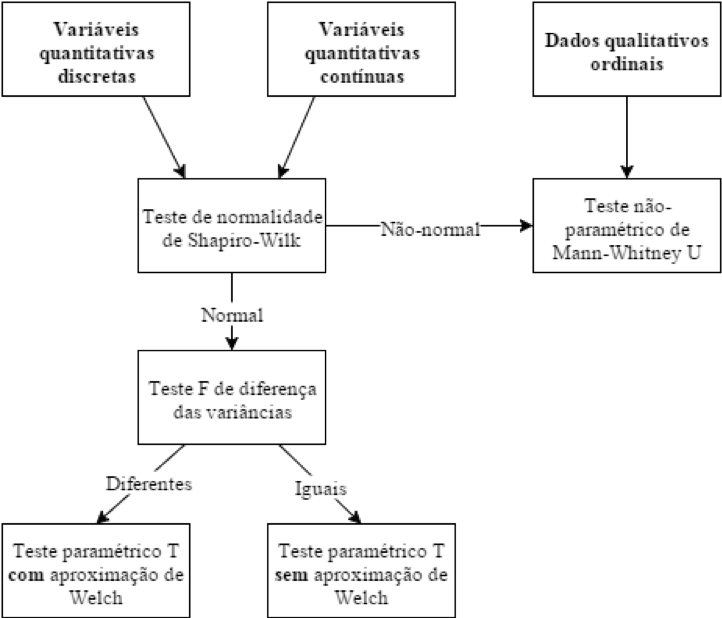
\includegraphics[scale=1.0]{./Figuras/fluxograma-tecnicas-moissa.png}
  \end{center}
  \legend{Fonte: \citeonline{moissa2016influencia}}
\end{figure}

Conforme o fluxograma na Figura \ref{fig:fluxograma-tecnica-moissa}, quando a variável é quantitativa (discreta ou contínua)
é realizado um teste de normalidade para verificar a distribuição dos valores. Se o resultado mostrar uma distribuição
normal é realizado o teste F para verificar a variância das amostras. Se o resultado do teste F mostrar que as variâncias
são diferentes a Aproximação de Welch será utilizada no teste T, caso contrário o teste T é aplicado sem a Aproximação de Welch.
Se o resultado do teste de normalidade mostrar uma distribuição não-normal é adotado o teste não paramétrico de
Mann-Whitney U. Este teste também é utilizado para todas as variáveis qualitativas ordinais, pois estas variáveis devem
ser analisadas através de testes não-paramétricos \cite{moissa2016influencia}.

Todos os testes mencionados estão disponíveis na ferramenta estatística R, que foi a ferramenta utilizada para todas as análises
realizadas nas Subseções a seguir.

\subsection{Análise do Questionário de Satisfação}\label{subsection:analise-questionario-satisfacao}

O Questionário de Satisfação aplicado ao final do Minicurso de Algoritmos tem o objetivo de identificar a percepção dos
alunos sobre a qualidade das recomendações e também da interface do Sistema de Recomendação em si. As questões do questionário
podem ser vistas no Apêndice \ref{ape:questionario-de-satisfacao} e possui 13 questões, divididas em 7 categorias. Todas
as questões foram selecionadas do questionário definido por \citeonline{pu2011user} (presente no Anexo \ref{ane:questoes-framework})
e traduzidas para o Português. Essas questões são afirmações nas quais os alunos devem se posicionar em uma escala de
Likert de cinco pontos, de "Discordo Totalmente" até "Concordo Totalmente". Também foi adicionada uma opção de "Não utilizei" para
os alunos que não utilizaram o Sistema de Recomendação (ou usaram sem perceber). A Tabela \ref{tab:questionario-satisfacao-respostas}
apresenta as respostas agrupadas dos alunos para cada uma das perguntas.

\begin{table}[h]
\footnotesize
\caption{Respostas ao Questionário de Satisfação}
\label{tab:questionario-satisfacao-respostas}
\centering
\begin{tabular}{|p{1.5cm}|p{1.8cm}|p{2.2cm}|p{0.6cm}|p{0.6cm}|p{0.6cm}|p{2.3cm}|p{2cm}|}
\hline
\textbf{Questão} & \textbf{Algoritmo}   & \textbf{Discordo tot.} & \textbf{-} & \textbf{-} & \textbf{-} & \textbf{Concordo tot.} & \textbf{Não utilizei} \\
\hline
\multirow{2}{*}{1}          & Tradicional & 2                   & 1                     & 2                         & 15                    & 11                  & 17           \\
                            & Proposta    & 0                   & 0                     & 6                         & 11                    & 7                   & 13           \\
\hline
\multirow{2}{*}{2}          & Tradicional & 1                   & 0                     & 5                         & 18                    & 6                   & 18           \\
                            & Proposta    & 0                   & 1                     & 7                         & 9                     & 9                   & 11           \\
\hline
\multirow{2}{*}{3}          & Tradicional & 2                   & 0                     & 8                         & 13                    & 8                   & 17           \\
                            & Proposta    & 0                   & 2                     & 4                         & 12                    & 8                   & 11           \\
\hline
\multirow{2}{*}{4}          & Tradicional & 1                   & 0                     & 5                         & 17                    & 6                   & 19           \\
                            & Proposta    & 0                   & 1                     & 8                         & 8                     & 10                  & 10           \\
\hline
\multirow{2}{*}{5}          & Tradicional & 3                   & 0                     & 4                         & 10                    & 10                  & 21           \\
                            & Proposta    & 0                   & 2                     & 9                         & 8                     & 6                   & 12           \\
\hline
\multirow{2}{*}{6}          & Tradicional & 3                   & 3                     & 3                         & 12                    & 8                   & 19           \\
                            & Proposta    & 0                   & 0                     & 5                         & 11                    & 10                  & 11           \\
\hline
\multirow{2}{*}{7}          & Tradicional & 2                   & 5                     & 4                         & 14                    & 9                   & 14           \\
                            & Proposta    & 1                   & 1                     & 7                         & 9                     & 7                   & 12           \\
\hline
\multirow{2}{*}{8}          & Tradicional & 0                   & 6                     & 3                         & 12                    & 9                   & 18           \\
                            & Proposta    & 0                   & 2                     & 8                         & 8                     & 6                   & 13           \\
\hline
\multirow{2}{*}{9}          & Tradicional & 2                   & 2                     & 7                         & 10                    & 7                   & 20           \\
                            & Proposta    & 0                   & 0                     & 11                        & 5                     & 8                   & 13           \\
\hline
\multirow{2}{*}{10}         & Tradicional & 1                   & 0                     & 10                        & 14                    & 4                   & 19           \\
                            & Proposta    & 0                   & 2                     & 4                         & 12                    & 8                   & 11           \\
\hline
\multirow{2}{*}{11}         & Tradicional & 2                   & 2                     & 6                         & 13                    & 5                   & 20           \\
                            & Proposta    & 0                   & 1                     & 6                         & 10                    & 8                   & 12           \\
\hline
\multirow{2}{*}{12}         & Tradicional & 4                   & 1                     & 6                         & 17                    & 2                   & 18           \\
                            & Proposta    & 0                   & 1                     & 5                         & 9                     & 10                  & 12           \\
\hline
\multirow{2}{*}{13}         & Tradicional & 2                   & 0                     & 6                         & 13                    & 12                  & 15           \\
                            & Proposta    & 0                   & 1                     & 4                         & 7                     & 14                  & 11           \\
\hline
\end{tabular}
\end{table}

Através das respostas dos alunos presentes na Tabela \ref{tab:questionario-satisfacao-respostas}, podemos perceber que
os alunos que utilizaram a abordagem Baseada em Conteúdo Tradicional tiveram mais respostas de "Discordo Totalmente" do
que os alunos utilizaram a abordagem Com Decaimento, com 25 para o algoritmo Tradicional e uma para a proposta desse trabalho.
Além disso, podemos perceber que 12 questões tiveram pelo menos um "Discordo Totalmente" para o grupo que utilizou o algoritmo
Tradicional e uma questão para o grupo que utilizou a Proposta Com Decaimento.

Com relação a resposta "Concordo Totalmente", tiveram 97 respostas para o grupo que utilizou o algoritmo Tradicional e 111
para o grupo que utilizou a proposta desse trabalho. O resultado das respostas "Não utilizei" mostram que os alunos responderam
que não utilizaram para apenas algumas perguntas e não para todas, sendo que para o grupo
que utilizou o algoritmo Tradicional o valor varia entre 17 e 21 alunos e para o grupo que utilizou a Proposta desse
trabalho variou entre 10 e 13 alunos. O fato desse valor ter variado tanto não foi esperado inicialmente, mas podemos afirmar que pelo menos 17 alunos do primeiro grupo e 10 alunos do segundo grupo
não utilizaram ter utilizado o Sistema de Recomendação. Ao comparar essa informação com os dados de acesso
dos alunos, que diz que 23 alunos do grupo Tradicional e 15 alunos do grupo Com Decaimento não acessaram nenhuma recomendação,
é provável que apesar de não terem acessado nenhuma recomendação os alunos perceberam o Sistema de Recomendação e analisaram
as recomendações recebidas.

As respostas dadas ao questionário de satisfação foram analisadas utilizando teste não paramétrico de
Mann-Whitney U para verificar se existe diferença estatisticamente significativa entre as respostas dos dois grupos (i.e., \textit{p} < 0.05).
As respostas de "Não utilizei" não foram consideradas nessa análise. O resultado das análises está presente no Apêndice
\ref{ape:analise-estatistica-questionario}. Essa análise mostrou que, apesar da aparente diferença nas respostas dadas
pelos alunos favorável à proposta desse trabalho, apenas uma questão apresentou uma diferença significativa entre as
respostas dos dois grupos. Isso se deve ao fato de ter mais respostas em "Discordo Parcialmente",
"Não Concordo e Nem Discordo" e "Concordo Parcialmente" para o grupo do algoritmo Tradicional do que para o grupo da
Proposta desse trabalho, com 248 para o primeiro e 217 para o segundo, que equilibrou os resultados dos dois grupos.

A única questão que apresentou diferença significativa foi a questão 12 (i.e., "Eu entendi porque os
itens foram recomendados para mim.") e foi favorável à proposta desse trabalho. A diferença significativa nessa questão
mostra que os alunos que utilizaram o algoritmo Com Decaimento puderam perceber melhor a relação entre os itens que acessaram
com os links que foram recomendados do que os alunos que utilizaram a abordagem Tradicional.

\subsection{Análise do uso do SR}\label{subsection:analise-uso-sr}

\section{Outras Análises}\label{section:outras-analises}

\section{Considerações sobre o capítulo}

Neste capítulo foi descrito o ambiente no qual o Sistema de Recomendação (SR) proposto será incorporado (\adaptweb) e definido o
experimento para a avaliação da proposta desse trabalho. Nos SRs desenvolvidos no \adaptweb, tanto para a proposta deste trabalho como para a abordagem
Baseada em Conteúdo tradicional que será utilizada como parâmetro, o perfil do usuário é composto pelo conjunto de palavras-chave de todos os itens acessados pelo usuário, das
cinco categorias apresentadas. Os itens a serem recomendados são os Links de Apoio, visto que os itens das outras categorias
são estruturados pelo professor e estão fortemente relacionados à conceitos específicos.

Utilizando como base as diretrizes propostas por \citeonline{pu2012evaluating} foi proposta uma interface para a apresentação das recomendações no \adaptweb,
com o objetivo de que os usuários tenham acesso direto as recomendações na tela principal do ambiente do aluno e entendam
melhor o porque aqueles itens foram recomendados. Como visto, essa interface será utilizada tanto pelo algoritmo proposto
quanto pela abordagem tradicional.

O experimento visa avaliar a experiência do usuário com o SR proposto no Capítulo \ref{chapter:proposta} em
comparação à abordagem Baseada em Conteúdo tradicional. O experimento acontecerá no ambiente
\adaptweb através de um minicurso de algoritmos desenvolvido no ambiente nos meses de
Abril e Maio de 2018. Ao final do minicurso os alunos receberão um questionário para responder sobre a sua experiência
ao interagir com o SR, que será adaptado do conjunto de questões definidas por \citeonline{pu2011user}. Ao final do
experimento, espera-se chegar a uma conclusão se existe diferença na percepção do usuário sobre a qualidade
das recomendações recebidas ao utilizar um SR Sensível ao Tempo, que se adapta as variações de interesse do
aluno, em relação a uma abordagem tradicional de recomendação.
